\section{Analysis}
\label{sec:formatting}
In this section we will go through the drawbacks and advantages of the evaluation metric with the help of two question-answer pairs projected on the same image. 
\begin{figure}[htbp]
  \centering
   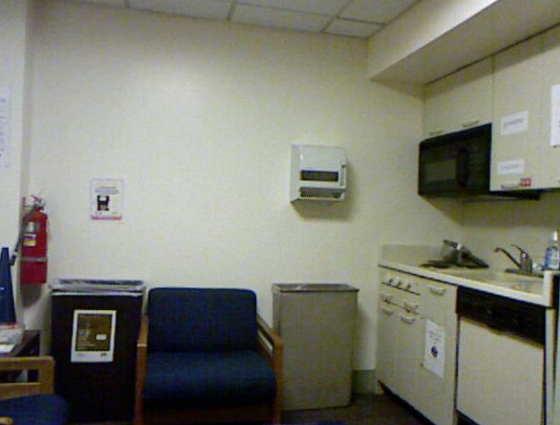
\includegraphics[width=0.75\linewidth]{sec/Images/image9.png}
   \caption{}
   \label{fig:onecol}
\end{figure}



Fig. 7 shows an image instance from DAQUAR dataset to which the BLIP question-answer model is applied. 
Fig. 8 presents two cases which includes the question asked, the prediction we get and the ground truth on the image.

\begin{figure}
    \centering
    \begin{subfigure}{0.5\textwidth}
        \centering
        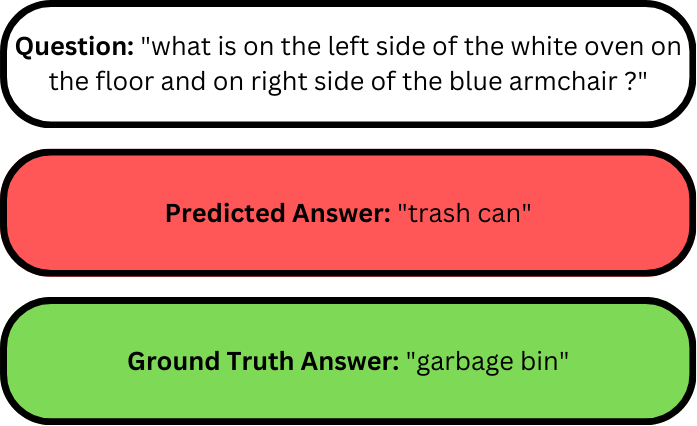
\includegraphics[width=0.5\textwidth]{sec/Images/image10.png}
        \caption{Case 1}
        \label{fig:sub1}
    \end{subfigure}
    \hfill
    \begin{subfigure}{0.5\textwidth}
        \centering
        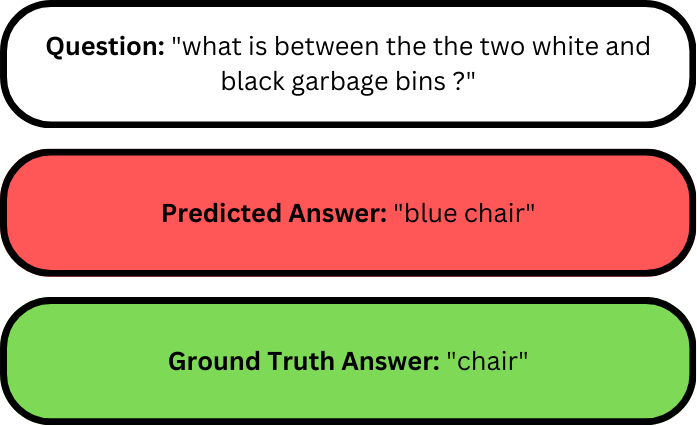
\includegraphics[width=0.5\textwidth]{sec/Images/image11.png}
        \caption{Case 2}
        \label{fig:sub2}
    \end{subfigure}
    \label{fig:whole}
\end{figure}


\subsection{Accuracy}
As evident from the results, the BLIP model exhibits relatively low accuracy. However, relying solely on accuracy metrics may not comprehensively assess the model's performance. As shown in the example above, strict matching between predicted and best ground truth results may overlook semantically similar answers, as explained below : \\
\begin{itemize}
    \item \textbf{Case 1}: The model predicted "trash can" while the ground truth was "garbage bin", resulting in a 0 accuracy score despite the similarity in meaning.
    \item \textbf{Case 2}: The model predicted "blue chair" while the ground truth was "chair", resulting in a 0 accuracy score despite the more detailed answer.
\end{itemize}


Hence, accuracy alone may not adequately reflect the model's effectiveness in capturing nuanced semantic relationships.

\subsection{BLEU Score}

The BLIP model's subpar accuracy underscores the importance of adopting nuanced evaluation metrics such as the BLEU score. Unlike traditional accuracy, BLEU considers n-gram overlaps, providing a more comprehensive understanding of the model's performance across diverse datasets.

\begin{itemize}
    \item \textbf{Case 1}: The model predicted "trash can" while the ground truth was "garbage bin", resulting in a 0 BLUE score despite the similarity in meaning because it checks for the n-gram overlaps.
    \item \textbf{Case 2}: The model predicted "blue chair" while the ground truth was "chair", resulting in a 0.5 BLUE score due to a small degree of overlap in the answer.
\end{itemize}

Thus, the BLUE score is better than the standard accuracy but is still insufficient because it does not take the semantic similarity into account.


\subsection{BERT Score}
\begin{itemize}
    \item \textbf{Case 1}: The model achieved a BERT Precision score of 0.90, indicating high semantic similarity between the model’s output (“trash can”) and the ground truth value (“garbage bin”).
    \item \textbf{Case 2}: The model predicted "blue chair" while the ground truth was "chair", resulting in a BERT Precision score of 0.83 due to high similarity.
\end{itemize}

Thus, as shown by the results, the BERT score is a highly valuable metric for assessing the performance of the model.

\subsection{WUPS Score}
\begin{itemize}
    \item \textbf{Case 1}: The WUPS score is good in case 1. The score is 0.76 at 0 threshold and 0.0076 at 0.9 threshold.
    \item \textbf{Case 2}: The WUPS does not provide a good score in case 2. The score is 0.11 at 0 threshold and is 0.011 at 0.9 threshold.
\end{itemize}

WUPS score provides us insight into the semantic similarity between our model’s output and the ground truth values in some cases, however, it is unable to capture the semantic similarity of the words in all the cases. 

\subsection{VQA Accuracy}
\begin{itemize}
    \item \textbf{Case 1}: VQA accuracy is 0.67 because the model’s output matched 2 answers out of the 10 available answers.
    \item \textbf{Case 2}: VQA accuracy is 0.33 because the model’s output matched exactly 1 answer of the 10 available answers.
\end{itemize}

VQA score provides a more accurate depiction of the model’s performance as compared to simple accuracy by comparing the predictions with all the available answers. However, it still does not take the semantic similarity into account, which is not ideal. 
%------------------------------------------------------------------------





